\section{Grading}
\label{benotung}
Click on the Grade tab (see Fig. \ref{benotung_uebungen} (1))

\subsection{Overview and Grading of the Activities}
\label{ben}

\begin{figure}[ht]
\begin{center}
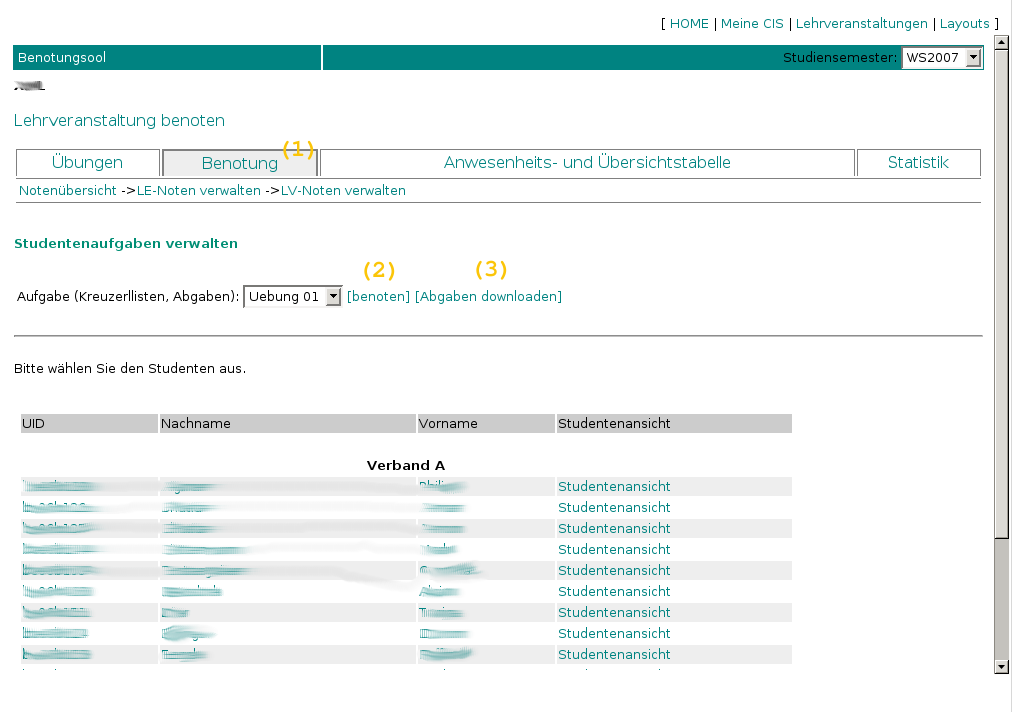
\includegraphics[width=1.0\textwidth]{benotungstool_benotung.png}
\end{center}
\caption{Grading Activities}\label{benotung_uebungen}
\end{figure}

Select an activity, assignment or checklist from the drop-down menu and click "'Grade"' (see Fig. \ref{benotung_uebungen} (2)).
A new page will open with a list of all the students and a grade box or check boxes for the checklist items, as well as the student upload file (see Fig. \ref {notenliste}).
Make your entries and save the page with the button at the bottom right. Close the page.

\begin{figure}[ht]
\begin{center}
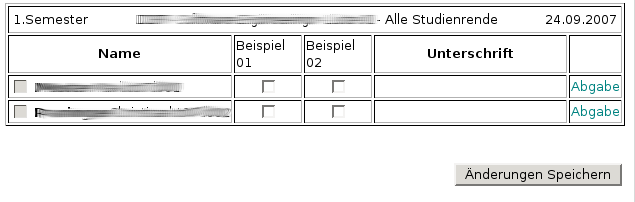
\includegraphics[width=0.7\textwidth]{benotungstool_notenliste.png}
\end{center}
\caption{Grade List}\label{notenliste}
\end{figure}


If there is a student upload for an assignment, a further link will be displayed next to the "'Grade"' link for downloading a ZIP file with all student uploads for this assignment (3).

By clicking on the name of a student, you can assign grades, checklists, participation points and notes for this student in detail. \footnote{The structure is essentially the same as the old "'checklist tool"'}

\subsection{Student View}
\label{studentenansicht}
You can display the student view for the students in your group by clicking on the "'Student View"' link (to the right of the name in the list). A new window will open displaying the student view of the selected student. In this window, you assume the identity of the student and can perform all the same functions there as the student. 

However, this function is only intended for overview/demonstration purposes. Always use the lecturer admin interface as described in section \ref{ben} to make changes to data (add/delete checklists)!

\subsection {Management of Teaching Unit Grades}
\begin{figure}[ht]
\begin{center}
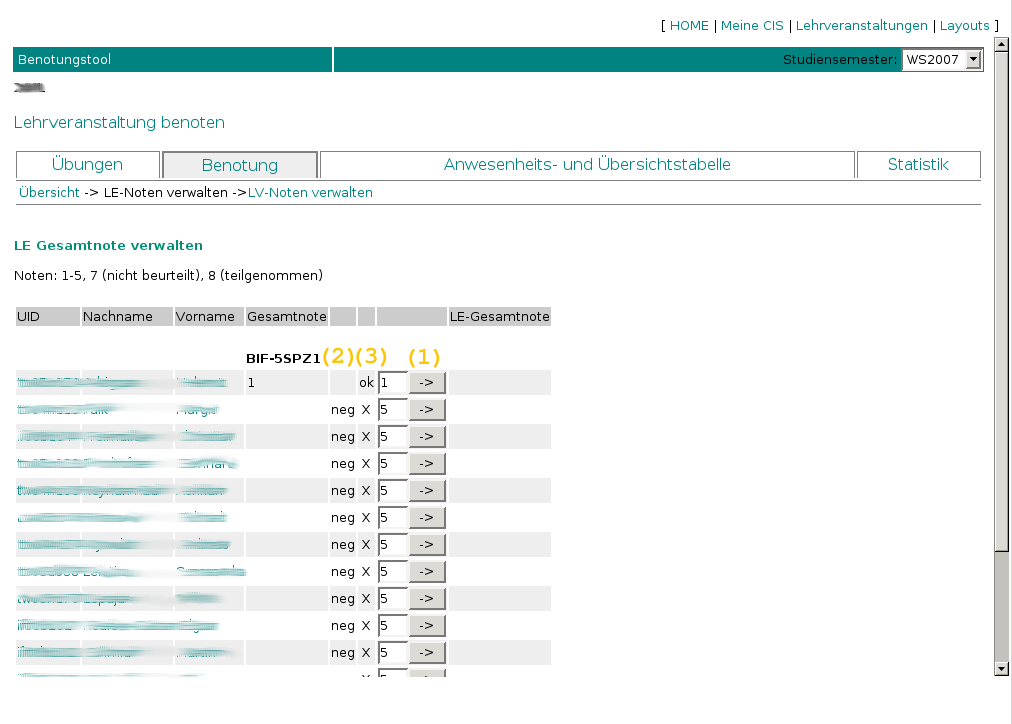
\includegraphics[width=1.0\textwidth]{benotungstool_benotung_le.png}
\end{center}
\caption{Grading Teaching Units}\label{benotung_le}
\end{figure}

A final grade for the teaching unit is calculated based on the grades of the individual activities, assignments and checklists using the point values you defined or the grading key in the case of checklists.
This score is rounded and suggested as the final grade for the teaching unit.
Verify/correct the suggested grades and accept them by clicking the '-$>$' - button.
(see Fig. \ref{benotung_le} (1))

Additional fields:
"'neg"' (2) in the column next to the calculated grade indicates that at least the required, defined positive grade is negative; "'ok"'/"'x"' (3) indicates whether all partial scores are available.

%\input{Final Grade}
%\newpage
